\section{Basic probability}
\section{Basic Probability Theory}
\begin{itemize}
\item Outcome --- Set of possible outcomes
\item Event  --- Subset of possible outcomes, an event is something which can happen or not happen
\item Distribution  ---  measure on the outcome space, just give the probability of each outcome
\item Independence  --- "Events that are unrelated", depends on the distribution
\end{itemize}

\subsection{Discrete Examples}
\begin{itemize}
\item Coin Flip: 
        \begin{itemize}
        \item Outcomes: $\left\{ H, T\right\}$
        \item Event:  If we toss a coin once, there are two possible events: $\{H\}$ and $\{T\}$; If we toss a coin twice, the event that the first toss is heads is $A = \{HH,HT\}$;  If we toss a coin three times, the event that the second toss is heads is $B = \{HHH, THT,HHT, THT\}$.
        \item Distribution: If we toss a coin, the possibility that it is H and the possibility that it is T are the same, that is $p(\left\{H  \right\})=p(\left\{ T \right\})=0.5$.%, $p(\left\{ H \right\})=0.2, p(\left\{  T\right\})=0.8$
        \end{itemize}
\item Rolling a Die:
        \begin{itemize}
        \item Outcomes:$\left\{ 1, 2, 3, 4, 5, 6\right\}$
        \item Event: some examples\newline
        		$E_{1}=\left\{ 3\right\}$--- rolling a 3\newline
                 $E_{2}=\left\{ 1, 3, 5\right\}$ --- rolling an odd number\newline
                 $E_{3}=\left\{ 2, 4, 6\right\}$ --- rolling an even number \newline
                 $E_{4}=\left\{ 1, 2\right\} $--- rolling either a 1 or 2
        \item Distribution: $p(\left\{1 \right\})=p(\left\{ 2 \right\})=...=p(\left\{ 6 \right\})= \frac{1}{6}$(most common case)\newline
        $p(\left\{ 1\right\})=\frac{1}{2}, p(\left\{ 2 \right\})=...=p(\left\{ 6 \right\})=\frac{1}{10}$ (for some special die)
        \item Independence: Given events $E_{1}$ and $E_{2}$, they are independent if \newline
        $p(E_{1} \bigwedge E_{2})=p(E_{1})p(E_{2})$(the probability that both events appear is equal to the product of the probability that one event appears)\newline
        $p(E_{1}|E_{2})=\frac{p(E_{1} \bigwedge E_{2})}{p(E_{2})}=p(E_{1})$ (the conditional probability of $E_1$ given the event $E_{2}$ is equal to the probability of $E_1$) 
        \item example of independence: The die roll 2 and 3 are independent; Events $E_2$ and $E_4$ are also independent:\newline
        $E_{2}  \bigwedge E_{4}=\left\{1,3,5\right\} \bigwedge \left\{1,2\right\} =\left\{1\right\}$\newline
        $p(E_{2} \bigwedge E_{4})=p(\left\{1\right\})=\frac{1}{6}$\newline
        $p(E_{2}) p(E_{4})=p(\left\{1,3,5\right\})p(\left\{1,2\right\})=\frac{1}{2}\frac{1}{3}=\frac{1}{6}$
        \end{itemize}
\end{itemize}

\subsection{Independent Copies}
\begin{itemize}
\item Coin Flip: 2 independent copies:\newline
$C_{1}=\left\{H,T\right\}, C_{2}=\left\{H,T\right\}\Rightarrow C_{1}\times C_{2}$\newline
\begin{tabular}{c|c|c} 
	& $H^{\operatorname{P_{H}}}$ & $T^{P_{T}}$ \\
	\hline$P_{H} H$ & $H H$ & $H T$ \\
	\hline$P_{T}T$ & $T H$ & $T T$
\end{tabular}
  \begin{itemize}
      \item Event: $\left\{HT,HT\right\} \Rightarrow $ exactly one head \newline
      $\left\{HT,HH,TH\right\} \Rightarrow $at least one head
      \item Distribution: $p((H,T))=p_{1}(H)p_{2}(T)$
      \item Generalized: K-coins \textbf{independent}. $\left\{H,T\right\}^{K}=\left\{K-tuples \ of  \  H,T\right\}$ \newline
      Distribution. $p((H,...,T))=p_{1}(H)...p_{k}(T)$ Can generalize this to infinite protucts as well. (Doesn't hold for dependent events)
   \end{itemize}
\end{itemize}

\subsection{Continuous Distributions}
\begin{itemize}
	\item Ex: Uniform Distribution on $\left[ 0,1\right]$ .\newline
	Outcomes: $\left[ 0,1\right]$ \newline
	Events: Ex: the event $\left[ 0,0.5\right]$ means random number $\leq$ 0.5 \newline
	            Ex: the event $\left[ 0,0.25\right] \bigcup \left[ 0.5,0.75\right]$ means random number less than $0.025$ or between $0.5$ and $0.75$\newline
 \begin{figure}[ht!]
	\centering
	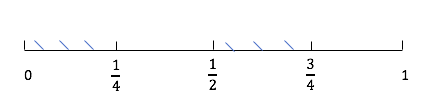
\includegraphics[width=.35\textwidth]{../figures/probability1.png}  
\end{figure}	      

	\item Distribution: \newline
	A distribution a rule which gives the probability of any event. \newline
	Properties to satisfy: if events $E_{1}, E_{2}, ..., E_{n},...  \mbox{satisfy that}  \ E_{i} \bigcap E_{j}= \varnothing $, then 
	\begin{enumerate}
	\item $ p(E_{1} \bigcup ... \bigcup E_{n} \bigcup ...) = \sum_{i=1}^{\infty}p(E_{j})$
	\item $p(E)=\int_{E} d_{x}$, "length of E" 
	\item examples 1: $E_{1}=\left[ 0,0.5\right] $
	$$
	P\left(E_{1}\right)=\int_{E_{1}} d_{x}=\int_{0}^{1 / 2} d x=\frac{1}{2}.
	$$
	\item examples 2: $E_{2}=\left[ 0,0.25\right] \bigcup \left[ 0.5,0.75\right]$
	$$p\left(E_{2}\right)=\int_{E_{2}} d x=\int_{0}^{1 / 4} d x+\int_{1 / 2} ^{3/4}d x=\frac{1}{4}+\frac{1}{4}=\frac{1}{2}
	$$
	\end{enumerate}	
 \begin{figure}
	\centering
	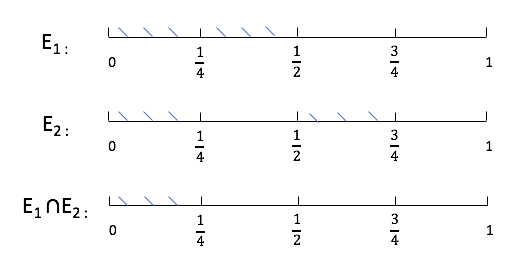
\includegraphics[width=.7\textwidth]{../figures/probability2.jpeg}  
\end{figure}
\item Independence: \newline
Two events $E_{1}, E_{2}$ are independent if \newline
$$p\left(E_{1} \cap E_{2}\right)=p\left(E_{1}\right) p\left(E_{2}\right)$$
For example,
$E_{1} \cap E_{2}=[0,0.5] \cap\left(\left[0, \frac{1}{4}\right] \cup\left[\frac{1}{2}, \frac{3}{4}\right]\right)$  	
$$
p\left(E_{1}\bigcap E_{2}\right)=\frac{1}{4}=\frac{1}{2} \cdot \frac{1}{2}=p\left(E_{1}\right) p\left(E_{2}\right)
$$

Frist two binary digits are like two independent coin flips. Every binary digit is like an independent coin flip, so we ca think of the random number as being an infinite sequence of coin flips. In general, we'll consider distribution defined by a probability density function p(x). The probability of an event is given by	$P\left(E\right)=\int_{E_{1}} p(x)d_{x}$
\begin{itemize}
\item Outcomes: $\left[ 0,1\right]$
\item Density function: $p(x)=1$ ($\int_0^1 p(x)=1$)
\end{itemize}
\end{itemize}


\subsection{Gaussian/ Normal Distribution}
 \begin{figure}[ht!]
	\centering
	
\includegraphics[width=.7\textwidth]{../figures/probability3.png}  
\end{figure}
\begin{itemize}
	\item Outcomes: 
	\item Events: Subsets of R
	\item Density function: $P(x)=\frac{1}{\sqrt{2\pi}} e^{-x^{2} / 2}$\newline
	         Means that for any event $E$,
	         $$
	         p\left(E\right)=\int_{E} \frac{1}{\sqrt{2 \pi}} e^{-x^{2} / 2} d x.
	         $$
	         
	 \item Cummulative distribution Function 
	 $$
	 F(x)=\int_{-\infty}^{x} p(t) d t=p(t<x)
	 $$
	 Note that $\lim_{x\rightarrow \infty} F(x)=1$.
\end{itemize}

\section{Random, Variable, Mean, Variance}
\begin{itemize}
\item Recall: 
\begin{itemize}
	\item Set if outcomes:  $\Omega$
	\item Event: Subset of outcomes: $E$
	\item Probability Distribution: $p(x)$
\end{itemize}
\subsection{Random Variable}
\item Defin: A random variable X is a function $X: \Omega \rightarrow S$ Here $ S=R, R^{d}$, but could be arbitrary.
 \item Ex: Rolling a die:
 \begin{itemize}
 	\item Outcomes: $\Omega={1,2,...,6}$
 	\item Events are subsets of $\Omega$
 	\item Distribution: $p(1)=p(2)=...=p(6)=\frac{1}{6}$
 	Suppose we roll the die, then if the die comes up d times, you win d dollars, minus 1 dollar if it's even. The amount you win is a random variable. \newline
 	$\begin{array}{l}
 		X_{1}: \Omega \rightarrow R\\
 		X_{1}(1)=1 \\
 		X_{1}(2)=1 \\
 		X_{1}(3)=3 \\
 		X_{1}(4)=3 \\
 		X_{1}(5)=5 \\
 		X_{1}(6)=5
 	\end{array}$ \newline
 	Can define multiple random variables on a single outcome space $\Omega$. 	
 \end{itemize}  
\item Ex: Rolling a die. If the die comes up d times, you get d dollars. If d is even, then you give a dollar to your friend.\newline
$X_{1} \leftarrow$ your winnings,
$X_{2}\leftarrow$ your friends winnings. \newline
$$
\begin{aligned}
	X_{2}: \Omega \rightarrow \mathbb{R}, & X_{2}(1)=0, \quad X_{2}(2)=1 \\
	& X_{2}(3)=0, \quad X_{2}(4)=1 \\
	& X_{2}(5)=0, \quad X_{2}(6)=1
\end{aligned}
$$
From here on out $\Omega$ will be fixed, we talk about different random variables on $\Omega$.
\subsection{Mean of  random variable}
\item Defin: Mean of a random variable $X$. \newline
Expectation of $X$: 
$$
\mathbb{E}[X]=\sum_{\omega \in \Omega} p(\omega) X(\omega)\left(=\int_{\Omega} X(\omega) p(\omega) d \omega\right)
$$
\item Ex: 
 $$\begin{aligned}
& \mathbb{E}\left[X_{1}\right]=\frac{1}{6}(1+1+3+3+5+5)=3 \\
& \mathbb{E}\left[X_{2}\right]=\frac{1}{6}(0+1+0+1+0+1)=\frac{1}{2}
\end{aligned}
$$
\subsection{Variance of  Random Variables}
\item Defin: Variance of a Random Variable $X$:  
$$
V[X]=\mathbb{E}\left[X^{2}\right]-\mathbb{E}[X]^{2}=\mathbb{E}\left[(X-\mathbb{E}[X])^{2}\right]
$$
\item Ex: 
$$
\begin{array}{l} V\left[X_{1}\right]=\mathbb{E}\left[X_{1}^{2}\right]-(3)^{2}\\
	= \frac{1}{6}\left(1^{2}+1^{2}+3^{2}+3^{2}+5^{2}+5^{2}\right)-9\\
	=\frac{1}{3}(1+9+25)-9\\
	=\frac{35}{3}-9=\frac{8}{3}\\
\end{array}$$ \newline
Variance measures "how much $X$ deviates from it's average".

 \begin{figure}
	\centering
	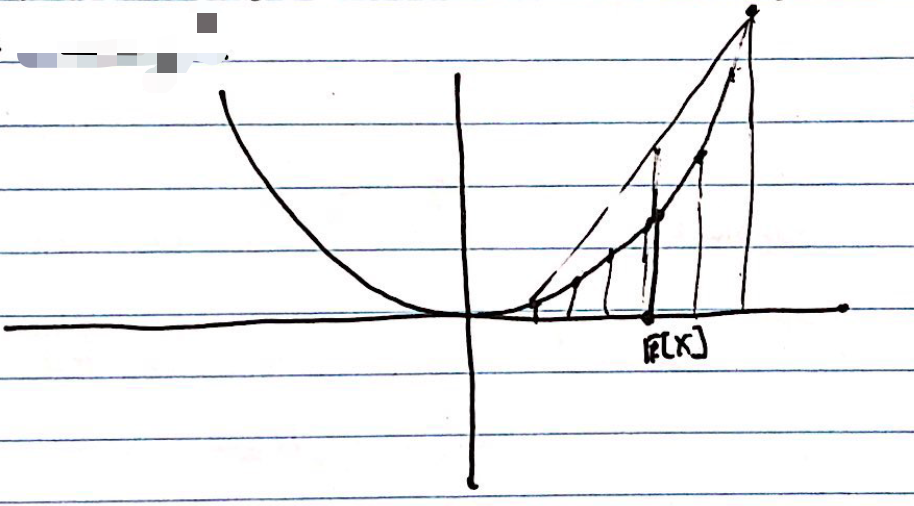
\includegraphics[width=.35\textwidth]{../figures/probability4.png}  
\end{figure}	

\subsection{Independenve of Random variables}
\item Defin:  Two random variables $X_{1},X_{2}$ are independent if for any $ \alpha, \beta,$
$E_{1}=\left\{w: X_{1}(\omega)<\alpha\right\}, E_{2}=\left\{w: X_{2}(\omega)<\beta\right\}$ are independent events.
\item Ex: $X_{1} , X_{2}$ are independent: if $(\alpha, \beta) \quad \alpha=4, \quad \beta=\frac{1}{2}$,
$$
\begin{array}{l} 
E_{1}=\left\{w: X_{1}(u)<4\right\}=\{1,2,3,4\} \\
E_{2}=\left\{w: X_{2}(\omega)<\frac{1}{2}\right\}=\{1,3,5\}
\end{array}
$$
$$
\begin{array}{l}
p\left(E_{1}\bigcap E_{2}\right)=p\left(E_{1}\right) p\left(E_{2}\right) \\
p(\{1,3\})=p\left(E_{1}\right) p\left(E_{2}\right)
\end{array}
$$

\subsection{Properties of E, V, Independence} 
\begin{itemize}
	\item If $X_{1}, X_{2}$ are random variable, then 
	$$
	\left(a_{1}X_{1}+a_{2} x_{2}\right)(w)=a_{1} x_{1}(w)+a_{2} x_{2}(w)
	$$
	$$\mathbb{E}\left[a_{1}X_{1}+a_{2} X_{2}\right]=a_{1}\mathbb{E}\left[X_{1}\right]+a_{2} \mathbb{E}\left[X_{2}\right]
	$$
	\item If $X_{1}, X_{2}$ are independent random variables, then 
	$$
	\mathbb{E}\left[X, X_{2}\right]=\mathbb{E}\left[X_{1}\right] \mathbb{E}\left[X_{2}\right]
	$$
	\item From this, we get if $X_{1}, X_{2}$ are independent,  	
	$$
	V\left[X_{1}+X_{2}\right]=V\left[X_{1}\right]+V\left[X_{2}\right]
	$$
	$$V\left[a_{1} x_{1}+a_{2} x_{2}\right]=a_{1}^{2} V\left[x_{1}\right]+a_{2}^{2} V\left[x_{2}\right]
	$$
\end{itemize}	

\end{itemize}

%
%\includepdf{HandWrittenNotes/Probability1.pdf}
%\includepdf{HandWrittenNotes/Probability2.pdf}
%\includepdf{HandWrittenNotes/Probability3.pdf}
%\includepdf{HandWrittenNotes/Probability4.pdf}
%\includepdf{HandWrittenNotes/Probability5.pdf}
%\includepdf{HandWrittenNotes/Probability6.pdf}
%\includepdf{HandWrittenNotes/Probability7.pdf}
%\includepdf{HandWrittenNotes/Probability8.pdf}
%\includepdf{HandWrittenNotes/Probability9.pdf}

